
\section{CLIP Embedding Space Analysis}
In this section, we present a detailed analysis of the CLIP embedding space. CLIP offers a pre-trained joint embedding space, enabling zero-shot vision-language tasks. However, there is still a \textit{modality gap} present in the CLIP embedding space \cite{MindGap}. This gap refers to a geometric property where image and text embeddings occupy distinct regions within the embedding space. We further analyze and demonstrate that the modality gap arises from an inherent ambiguity in matching visual and linguistic embeddings. Empirically, we show that integrating subregion image information with global information can reduce the gap between linguistic and visual representations. Additionally, we explore the disparity between CLIP's text and image representations, conducting an empirical study that reveals the difference follows a Gaussian distribution. These findings inspire our subsequent method design.
  
%\subsection{Preliminary of Modality Gap}
% -----------------------------------------------------------------------
% CLIP通过在大规模数据上的contrastive language-Image pretraining获得了joint embedding space,但这个joint embedding space上仍然有modality gap. modality gap指在clip embedding space中,text embedding和image embedding中间仍然存在gap。这种gap存在的原因是CLIP的预测始终会存在mismatch image text pair,这些mismatched pair的存在使得contrastive loss有保留这样的modality gap(有mismatch data的前提下,保留一定的modality gap使得contrastive loss达到global minimum)
% -----------------------------------------------------------------------
%CLIP obtain a joint embedding space by contrastive language-Image pretraining on a large dataset of images and their corresponding text descriptions. However 

\begin{figure}[t!]
  \centering
  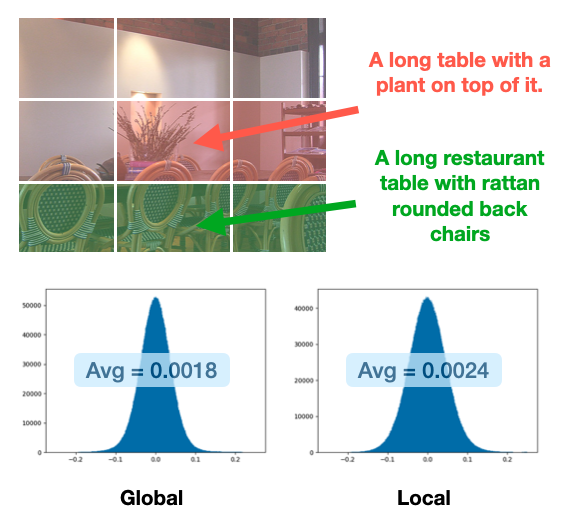
\includegraphics[width=0.35\textwidth]{AnonymousSubmission/LaTeX/asserts/ana_fig.png}
   \caption{The upper half of this figure is an example of the misalignment in paired image and text description. The lower half of this figure is the distribution of modality gap between text representation and global / local image representation respectively.}
    \label{figure:ex}
\end{figure}


\begin{table}[t]
\small
\centering
\tabcolsep=2pt
\begin{tabular}{c|ccc}
\toprule
\toprule
\multirow{2}{*}{} & \multicolumn{3}{l}{Pair Cosine Similarity} \\
                         & Mean        & Max        & Min        \\ \hline
 Global representation           & 0.330       & 0.446      & 0.228      \\ \hline

Mix representation             & 0.352       & 0.422      & 0.242      \\ \toprule
\end{tabular}
\caption{In this table, we show the mean, max and min value of similarity between text feature and global/mix feature. We find that after adding subregion information, the mean, max and min value all increase. This observation shows that introducing subregion image information benefit the alleviation of modality gap.}
\label{table:subregion}
\end{table}

\subsection{Modality Gap of CLIP Representations}
% \label{analysis:subregion}
% -----------------------------------------------------------------------
% modality gap的成因是mismatch pair。我们认为模型预测mismatch pair始终存在难以去除的原因是image和text两种模态表达的信息原本就是不对等的。具体地:1. 在annotation中认为是pair的image和text,text往往也并不描述image中的所有信息;2. text对图片描述了的部分,也难以避免歧义的发生;3. 并且对于同一个图片,也往往有多种进行文字描述的方法都是正确的,这些描述可能侧重图片的不同区域。这样的misalignment是固有的,因此是难以避免的。
% -----------------------------------------------------------------------

As demonstrated in \cite{MindGap}, the modality gap phenomenon is primarily caused by the presence of mismatched text-image data during pre-training, further exacerbated by the contrastive learning objective employed in CLIP. However, we observe that even correctly paired image-text may exhibit different semantic contents due to several reasons, including 1) incomplete image description by text; 2) ambiguity in text interpretation; 3) diverse valid descriptions with varying focus on image subregions. An example is illustrated in Figure~\ref{figure:ex}.
% Such modality misalignment is inherent, thus is hard to avoid. 
% -----------------------------------------------------------------------
% 基于这样的(mismatch image-text pair)的性质,我们可以利用subregion减弱modality gap带来的问题。我们假设对于某个具体地text description,一些subregion可能相比于global image有更小的gap。为了验证这个假设,我们进行了一些统计。我们计算global-text similarity和subregion-text similarity,取高的一个认为是匹配上了,我们发现有33%的subregion成功匹配上了。这样的结果验证了一些情况下subregion能有助于缩小modality gap
% -----------------------------------------------------------------------
%Based on the of characteristics, 
% we are able to alleviate the problems caused by modality gap by integrating CLIP visual feature with image subregion information. Given that the text description does not provide comprehensive representation of image and may focus on subregions of image, 
Consequently, we observe that certain subregions of an image typically exhibit a smaller modality gap with a specific text description, as illustrated in Figure~\ref{figure:ex}. To validate this characteristic, we conduct a statistical analysis on the MSCOCO validation set. Specifically, we calculate the cosine similarity between the visual and text features, where the visual features are obtained from the global CLS token or the last layer of the ViT encoder representing the subregions. The results indicate that in $\mathbf{33\%}$ of cases, one of the subregion features has a higher similarity than the global one.

%and embedded caption, visual patch feature and embedded caption feature. The visual patch features are from last layer of CLIP ViT encoder.
% the global-image-to-text similarity and subregion-to-text similarity. 
%A text description is said to be matched with the subregion if the similarity score of visual patch feature is higher, and vice versa. 

%We find that $\mathbf{33\%}$ of subregion representation successfully match with the text description. The results demonstrate the image subregion information may bring benefits to alleviate the modality gap. However, there still are $67\%$ cases the global representation achieve higher similarity score. 
%Consider that, we combine the global image representation and the local image representation by adding them together, and defined it as mix representation. We eval the similarity score between text representation and global/mix representation and show the results of mean, max and min score in Table~\ref{table:subregion}. We find that integrating subregion information leads to increase in mean score. This observation shows that introduce subregion image information benefit the alleviation of modality gap.

Motivated by the above observation, we propose integrating the global and subregion representations by adding them together. We evaluate the similarity scores between text features and their corresponding subregion-augmented image representations. As illustrated in Table~\ref{table:subregion}, our augmented image embeddings achieve higher similarity scores when compared with corresponding text embeddings without any fine-tuning, effectively reducing the modality gap.
% Specifically, we add the subregion representation to the global image representation. 
%The details will be presented in the \textit{Sub-region Feature Aggregation} section.
%As shown in our experiments, our sub-region augmented image embeddings achieve higher cosine similarity scores when compared with corresponding text embeddings without any fine-tuning.
% Below we will introduce our subregion-augmented embedding representation and a noise injection strategy to learn the mapping from image to text modality without paired data. 

\subsection{Distribution of Modality Gap}
% \label{analysis:Distribution_of_Modality_Gap}
We further investigate the distribution of the modality gap through an empirical study on the MSCOCO validation set. Specifically, for each image with its caption, we compute the difference between the image and text embeddings. We calculate these differences separately for the global image feature and the subregion feature. Given these differences, we pool all the feature dimensions together and compute a histogram and mean of the dimension-wise differences between the two modalities. As depicted in the lower half of Figure~\ref{figure:ex}, we observe that the mean of the gap distribution is close to zero, and the overall distribution resembles a Gaussian distribution for both global and subregion representations. Based on this observation, we adopt a unimodal learning strategy that involves Gaussian noise injection with the text features. This strategy allows us to mimic the image features in the cross-modal inference stage. For a more formal description of our analysis, please refer to the supplementary material.


%We have text modality representation $T^i \in \mathbb{R}^D$ and vision modality representation. To be noticed, for vision modality we have two set of representation: the global embedding representing the overall information and the patch embeddings representing the image subregions information. The global embedding is $I_c^i \in \mathbb{R}^D$, and the patch embedding is $I_p^i \in \mathbb{R}^{N \times D}$. Both global embedding and local embedding are obtained by CLIP. $D$ is the dimension of CLIP embedding and $N$ is the sequence length of CLIP. $i \in \{1, 2, ... , num\_samples\}$

%For paired images and text descriptions, we evaluate the gap between text representation and both global and patch image representation. For each image-text pair, we compute $G^c_i = T^i - I_c^i$ and $G^p_i = repeat(T^i, N) - I_p^i$. $G^c_i \in \mathbb{R}^{D}$, $G^p_i \in \mathbb{R}^{N \times D}$.

%We can check the overall distribution over all $D$ dimension. In this case, we treat data in all dimension equally. We compute the mean over all image-text pairs and draw the histgram of the data distribution. Thus we compute mean of the gap distribution for global vision and language representation as $Avg_{(i, d)} (I_c^i[d])$, and the gap for local vision and language representation as $Avg_{(i, s, d)} (I_p^i[s][d])$. $s \in [N], d \in [D]$ The results are shown in the lower half of  Figure~\ref{figure:ex}.

%The mean of the gap distribution between language and both global and local representation are close to zero. In Figure we sample $5e6$ example data and show the distribution, which is close to a Gaussian distribution. Based on this characteristic, we assume the modality gap distribution conforms to the Gaussian distribution. We are able to make the text representation closer to image representation by adding an appropriate Gaussian distribution.

\begin{figure*}[t!]
  \centering
  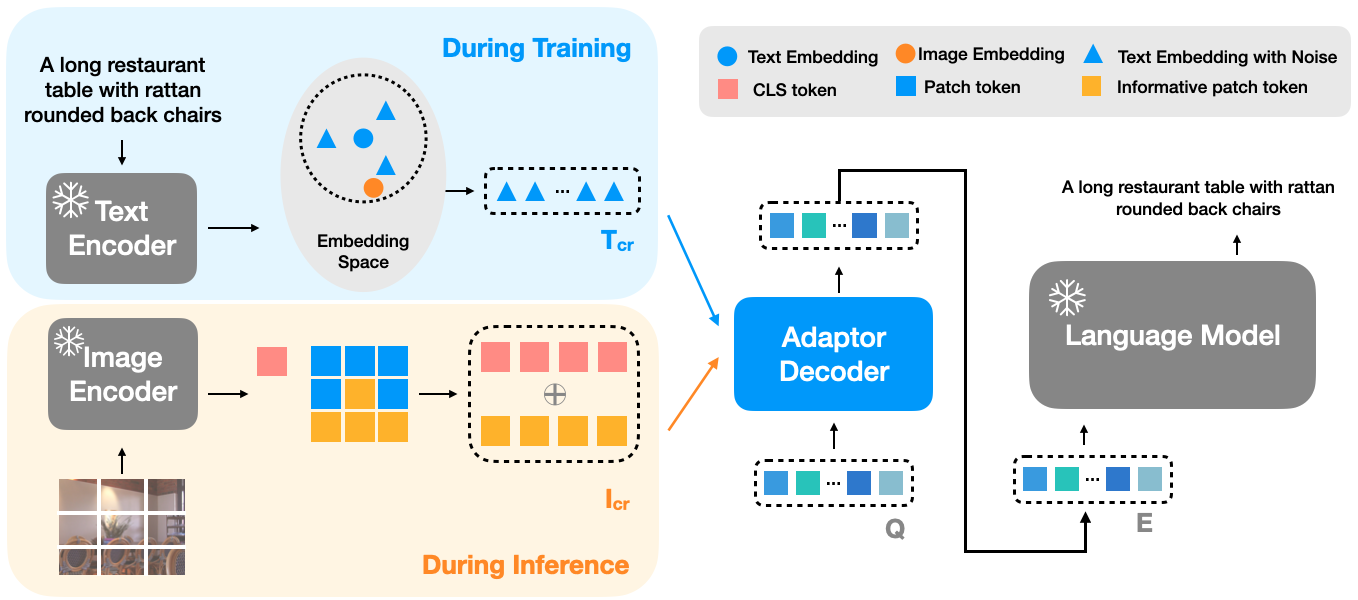
\includegraphics[width=0.7\textwidth]{AnonymousSubmission/LaTeX/asserts/new_pipeline.png}
   \caption{\textbf{An overview of MacCap pipeline.} MacCap learns to generate text based on region noise injected CLIP text feature in text reconstruction training. During inference, MacCap can generate caption without paired data in training. The CLIP and language model are kept frozen in both stages. }
    \label{figure:pipeline}
\end{figure*}
